\section{Introduction}

\todo[inline]{shorten and rephrase the CDC part.}
\todo[inline]{Need a discussion on related work, including RT papers, GP papers \protect\cite{nghiemetal16gp}, especially for buildings.}

Machine learning and control theory are two foundational but disjoint communities. Machine learning requires data to produce models, and control systems require models to provide stability, safety or other performance guarantees. Machine learning is widely used for regression or classification, but thus far data-driven models have not been suitable for closed-loop control of physical plants. The challenge now, with using data-driven approaches, is to close the loop for real-time control and decision making.

Consider a multivariable dynamical system subject to external disturbances. The first and foremost requirement for making any decision is to obtain the underlying control-oriented predictive model of the system. With a reasonable forecast of the external disturbances, these models should predict the state of the system in the future and thus a predictive controller based on Model Predictive Control (MPC) can act preemptively to provide a desired behavior. In particular, MPC has been proven to be very powerful for multivariable systems in the presence of input and output constraints, and forecast of the disturbances. The caveat is that MPC requires a reasonably accurate physical representation of the system. This makes MPC unsuitable for control of complex plants such as natural gas processing, oil refineries, boilers, manufacturing plants, and buildings where the user expertise, time, and associated sensor costs required to develop a model are very high \cite{Sturzenegger2016,vzavcekova2014}.

There are two main reasons for model complexity. 
(1) The prime contributor is the change in model properties over time. Even if the model is identified once via an expensive route, as the model changes with time, the system identification must be repeated to update the model. Thus, model adaptability or adaptive control is desirable for such systems. 
(2) A secondary reason is the model heterogeneity which further prohibits the use of model-based control. For example, unlike the automobile or the aircraft industry, each building is designed and used in a different way. Therefore, this modeling process must be repeated for every new building. 
Due to aforementioned reasons, the control strategies in such systems are often limited to fuzzy logic rules that are based on best practices. 

The question now is, can we employ data-driven techniques to reduce the cost of modeling, and still exploit the benefits that MPC has to offer? We therefore look for automatic and data-driven approaches to control that are also adaptive, scalable and interpretable. We solve this problem by bridging the gap between Machine Learning and Predictive Control.

\subsection{Challenges in bridging machine learning and controls}
\label{SS:practical_challenges}

The central idea is to obtain control-oriented models using machine learning or black-box modeling, and formulate the control problem in a way that receding horizon control (RHC) can still be applied and the optimization problem can be solved efficiently.

It is important to note that the standard machine learning regression used for prediction is fundamentally different from using machine learning for control synthesis. In the former, all the inputs to the model (also called regressors or features) are known, while in the latter some of the inputs that are the control variables must be optimized in real-time for desired performance. 
We next discuss the practical challenges in using machine learning algorithms for control.

\noindent \textbf{(1) Data quality:} Most of the historical data that are available from complex systems like buildings are based on some rule-based controllers. Therefore, the data may not be sufficient to explain the relationship between the inputs and the outputs. To obtain richer data with enough excitation in the inputs, new experiments must be done either by exciting the inputs randomly or by a procedure for optimal experiment design (OED) \cite{Emery1998,Fedorov2010}. This paper proposes the use of GP i.e.~the estimate of variance in GP predictions to recommend control strategies for OED.

\noindent \textbf{(2) Computational complexity:} Depending upon the learning algorithm, the output from a learned model is a non-linear, non-convex and sometimes non-differentiable (eg.~Random Forests \cite{Friedman2001}) function of the inputs with no closed-form expression. Using such models for control synthesis where some of the inputs must be optimized can lead to computationally intractable optimization. Our previous work uses an adaptation of Random Forests which overcomes this problem by separation of variables to derive a linearized input-output mapping at each time step \cite{JainACC2017,JainCDC2017}.
This paper uses Gaussian Processes (GP) for receding horizon control where the output mean and variance are analytical functions of the inputs, albeit non-convex.

\noindent \textbf{(3) Performance guarantees and robustness:} A desired characteristic for closed-loop control is to provide performance guarantees. This becomes hard when a black-box is used to replace a physical model. However, it is possible to provide probabilistic guarantees with a learning algorithm based on Gaussian Processes. GPs allow us to define chance constraints or account for model uncertainty in the cost while solving the optimization problem. This helps bound the performance errors with high confidence. Handling disturbance uncertainties or robustness to sensor failures in this framework is part of our on-going work and is thus excluded from this paper.

\noindent \textbf{(4) Model adaptability:} It is often the case that the model properties change with time, and thus, the learned model must also be updated when required. The traditional mode of system identification, done repeatedly, can be time and cost prohibitive, especially in the case of buildings. In this paper, we discuss the approach for evolving GP models that allows us to update the model from one season to another.

%\noindent \textbf{(5) Interpretability of control decisions:} Besides the accuracy of synthesizing control strategies with machine learning in the loop, we are also interested in solutions that are interpretable and trustworthy. Thus, the DPC recommendations should have traceability so they can be verified to be stable and safe. This direction of research also forms part of our on-going work.

\subsection{Overcoming practical challenges}
To address these challenges, we can take two different approaches based on how machine learning is used to learn the models.

\noindent \textbf{(1) Mix of black-box and physics-based models:} In this approach, we use machine learning to learn only the dynamics of a sub-system or to model uncertainties in the dynamics. An example of former is in the use of machine learning for perception and model-based control for low-level control in self-driving cars \cite{Urmson2008}. Examples on learning uncertainties in the models include \cite{Berkenkamp2015,Desaraju2016}.

\noindent \textbf{(2) Fully black-box models:} The full dynamical model can also be obtained using only machine learning algorithms. This deviates from the traditional notion of system identification where a physics-based structure is assumed to begin with. An example would be fully autonomous control using camera vision where control actions are mapped to raw image pixels \cite{Bojarski2016}. The catch here is that, prior to learning, sufficiently large data could be generated by running the car in simulations.

For the application to building control in context of Demand Response, where there is a massive cost to physical modeling, this paper explores the latter route to bypass the modeling difficulties as summarized in \cite{Sturzenegger2016}. The model-free approach allows to scale this methodology to multi-building campus and in general to m   any more applications like control of autonomous systems.

\begin{figure}[!t]
	\centering
	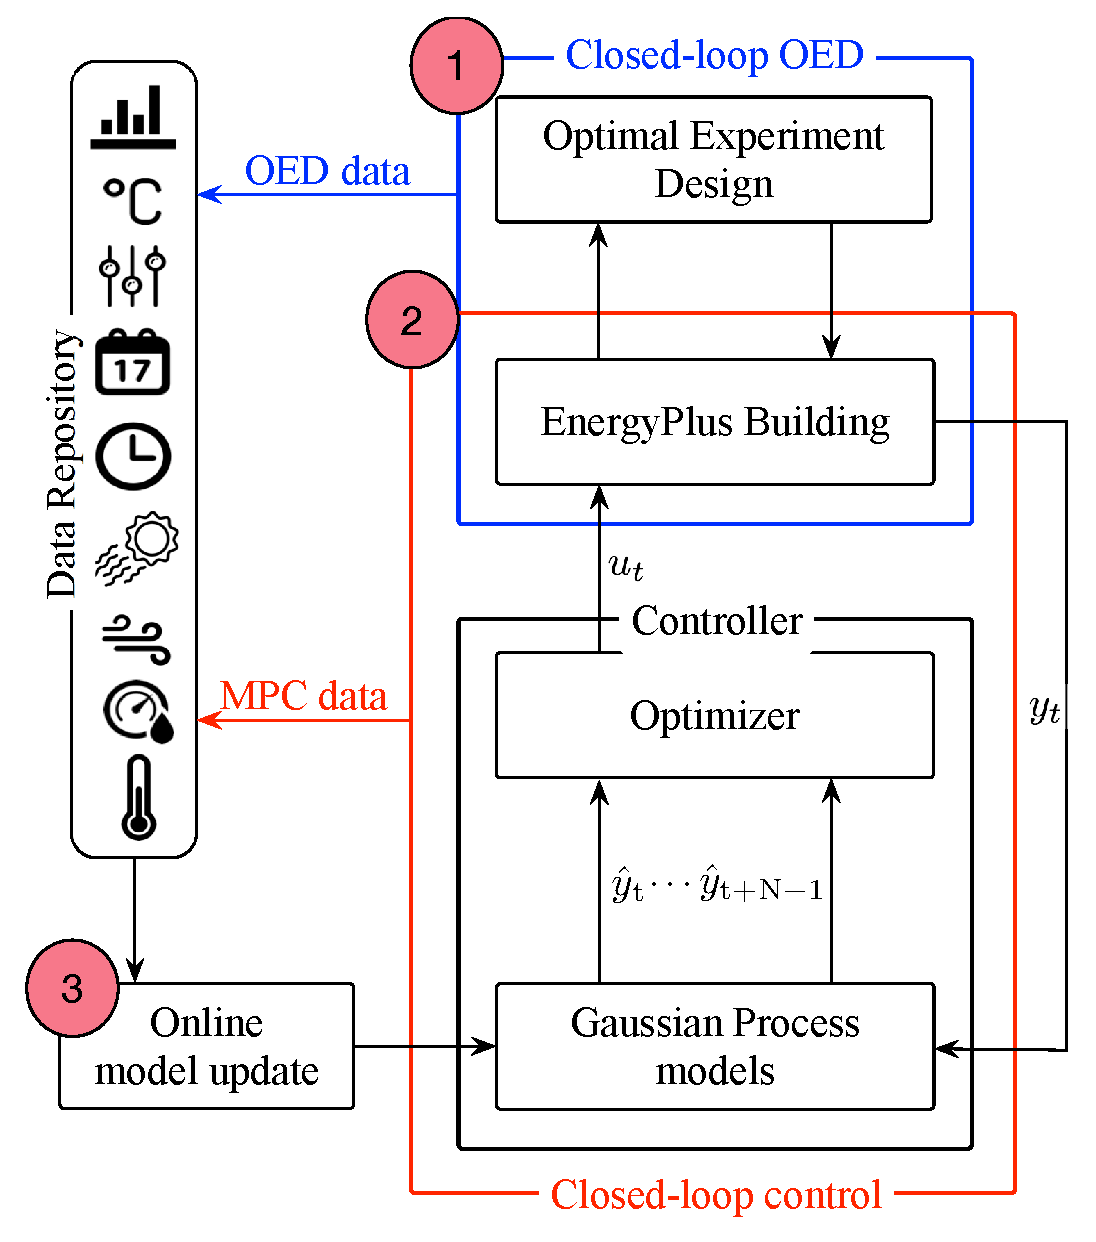
\includegraphics[width=1\linewidth]{figures/overview.eps}
	\caption{Paper organization and contributions}
	\captionsetup{justification=centering}
	\label{F:intro}
\end{figure}

\subsection{Contributions}

\todo[inline]{revisit when case study is ready}
\todo[inline]{Highlight contributions better and more strongly (here and in each section). Do not create the impression that we are ony applying existing methods.  For example, for OED, do not write as if we only apply informatics theoretic approach. Write that the original papers only use this approach for batch selection in sensor placement, while we develop sequential approach for OED.  Emphasizing the differences between our work and others.}

This paper attempts to answer the aforementioned practical challenges using fully black-box models based on Gaussian Processes.
This paper has the following contributions.
\begin{enumerate}
	\item The first part of the paper formalizes the problem of optimal experiment design using GPs. OED is particularly beneficial when limited data are available. We show that under operation constraints, OED based on maximizing information gain or maximizing variance can be used to recommend control strategies for exciting the system. These strategies provide more informative data and therefore more accurate models.
	\item We  then use the dynamical GP model learned from OED for real-time closed-loop receding horizon control where we formulate the MPC problem as a stochastic optimization problem.
	\item We apply the Bayesian approach to update the GP model as new data are generated by running the GP-based controller in a closed-loop with the physical system. Here, we again maximize the information gain to select the best subset of data to update the model as new data are available.
\end{enumerate}
An overview of the organization is shown in Fig.~\ref{F:intro}.
We apply all three methods to large-scale buildings in EnergyPlus \cite{Deru2011}. In the context of load curtailment for Demand Response, we apply OED to recommend control strategies to learn a model, fast and accurately. We show that MPC with GPs can provide the desired load curtailment with high confidence; maximum \(2.7\%\) error. After running the controller for a month, we relearn to update the GP model for a better performance, thus avoiding the need for a functional test in a new season.

%%% Local Variables:
%%% mode: latex
%%% TeX-master: "main"
%%% End:
